\chapter{Solving spin-glass problems using tensor networks}
\chaptermark{Solving spin-glass problems}

\label{chapter:tn}

Benchmarking quantum annealers requires adequate algorithms for providing
baselines for the obtainable solutions. While there exists a plethora of
general-purpose optimization algorithms, one might hope to achieve better
results by exploiting the topology of the problem's underlying graph and thus
locality therein. In this chapter, we describe a recent, tensor network-based
algorithm \cite{tn} for finding the low-energy spectrum of Ising spin-glasses,
designed for problems defined on Chimera-like quasi-two-dimensional graphs. The
algorithm exploits the sparsity and locality of the Chimera graph by
representing the Boltzmann distribution of spin-glass as a tensor network,
whose approximate contraction can be used for computing marginal probability
distributions. This procedure can then be combined with the well-known branch
and bound algorithm to iteratively select the most promising partial solutions,
finally producing an approximation of the low-energy spectrum.

\section{Exploring the probability space}

In the algorithm we are going to present in this chapter, we perform the search
in the probability space rather than in the energy space. This physics-inspired
approach is closely tied to the quantum computing paradigm. To explain why, let
us begin by replacing classical Ising Hamiltonian $H(s)$ with its quantum
counterpart $\mathcal{H} = H(\boldsymbol{\sigma}^{z})$ (i.e. replacing each
variable $s_{i}$ with a Pauli operator $\ssigma_{z}$ acting on the $i$-th spin.
Naturally, there exists a one-to-one correspondence between the eigenstates of
$\mathcal{H}$ and the possible classical states. If one now wishes to
find the low-energy spectrum of size $k \ll 2^{N}$, the task is equivalent to
finding the $k$ most probable states according to the Gibbs distribution $\rho
  \sim \exp(-\beta \mathcal{H})$. One way to achieve this is to prepare the
system in a Gibbs state:
\begin{equation}
  \ket{\rho} \sim \sum_{\mathbf{s}} \exp(-\beta \mathcal{H}/2)\ket{\mathbf{s}}
\end{equation}
and then perform a measurement. If repeated multiple times, this procedure
would yield the desired low-energy spectrum with high probability.

While the above procedure is useful conceptually, it clearly cannot be directly
used on a classical computer, as it would require preparing a dense vector of
$2^{N}$ elements. Instead, in our algorithm we represent the Gibbs distribution
approximately via a suitable tensor--network. Then, instead of performing a
quantum measurement, we extract the needed information by traversing the
probability tree using the branch-and-bound method. In what follows, we
describe the procedure in detail, starting with the branch-and-bound
part.
%\todo[inline,color=SkyBlue]{Mention the other Chimera-specific algorithm}

\section{Branch and bound}
Let us first consider an Ising spin-glass problem defined on a square lattice,
as depicted in Fig. \ref{fig:lattice-and-border}. The state space of such a
system can be viewed as a tree, in which $k$-th level contains all partial
configurations $(s_1, \ldots, s_k)$. This representation allows one to explore
the state space incrementally in search for low energy states, and possibly
prune the less promising branches. In the approach described here, we use
marginal probability $p(s_1, s_2, \ldots, s_k)$ as a criterion for deciding
which partial configurations are most promising. More precisely, we explore the
solution tree in a top-down manner, keeping at most $M$ states at $k$-th level
and branching them into $2M$ new partial configurations at level $k+1$. The
new marginal probability distributions can be computed using the following formula:
\begin{equation}
  \label{eq:conditional-prob}
  p(s_1, s_2, \ldots, s_k, s_{k+1}) = p(s_1, s_2, \ldots, s_k)p(s_{k+1}|, s_1, \ldots, s_k)
\end{equation}
The parameter $M$ can be made iteratoin dependend by keeping only the states
whose marginal probability divided by the maximal probability is larger than
sum \emph{probability cutoff} $\delta_{p}$.

We can exploit the locality of the problem by observing that conditional
probability in \eqref{eq:conditional-prob} of configuration in the region $X =
  (1, 2, \ldots, k)$ depends only on configuration on the border $\partial X$ comprising those spins that directly interact with the region
  $\overline{X} = (k+1, 2, \ldots N)$. For a detailed explanation of why this is the case
  we refer the reader to Section \ref{sec:probability} in the Appendix.

\begin{figure}
  \centering
  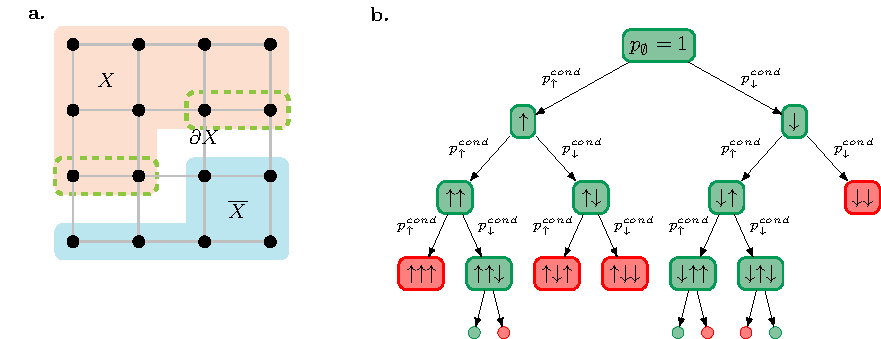
\includegraphics[width=\textwidth]{figures/squarelattice.pdf}
  \caption{\textbf{a.} An example Ising spin--glass  of 16 spins on a square lattice. The conditional probability for spins in the region $\overline{X}$ conditioned with a given configuration of spins in the region $X$ depends only on part of the configuration on the border $\partial X$. \textbf{b.} A fragment of the state space tree. States kept at each
    level are marked with green, and the pruned branches are marked with red.}
  \label{fig:lattice-and-border}
\end{figure}

Before discussing how probabilities in \eqref{eq:conditional-prob} can be
computed, let us first extend the above approach to the more general case of a
quasi-two-dimensional graph, i.e. one in which nodes can be grouped into
\emph{clusters} forming a two-dimensional square lattice (see Fig.
\ref{fig:clustering}). One can easily see, that again we can construct a
tree-like structure representing state space, this time considering joint
configurations of spins in a single cluster. Therefore, for most of the time,
we might "forget" the underlying spin-glass structure and consider square
lattices in which spin clusters act like higher-dimensional systems.
Furthermore, by the same argument, it is clearly visible that our approach is
not limited to the Ising systems, but could be also used for systems of higher
dimensions.

\begin{figure}
  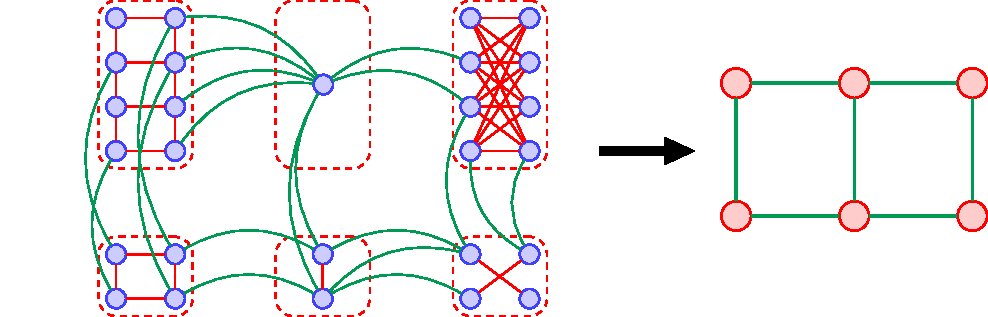
\includegraphics[width=\textwidth]{figures/clustering}
  \caption{Grouping spins into clusters in a quasi-two-dimensional graph. Here, spins in
    the original graphs are grouped together to form a square lattice. Each site in
    the new lattice then effectively serves as a higher-dimensional system.}
  \label{fig:clustering}
\end{figure}

% A central object considered in our algorithm is the probability distribution
% $\exp[-\beta H(\mathbf{s})]$, which we approximate using a PEPS-equivalent
% tensor network, whose detail will be described shortly. Contracting such a
% network can give the probability distribution of any full configuration, as
% well as the marginal probabilities.

% \begin{equation}
%   p(s_1, s_2, \ldots, s_k) \sim \tr[\mathcal{P}_{(s_1, \ldots, s_k)} e^{-\beta H(\mathbf{s})}]
% \end{equation}

\section{PEPS network construction}
We begin the construction of a PEPS network for a quasi-two-dimensional graph
by considering two spins at sites $i$ and $j$ connected by an edge $J_{ij}$.
This edge can be decomposed as:

\begin{equation}
  e^{-\beta J_{ij}s_i s_j} = \sum_{\gamma = \pm 1} B^{s_{i\phantom{j}}}_\gamma C^{s_j}_\gamma
\end{equation}
where
\begin{equation}
  \label{eq:decomposition}
  B^{S_i}_\gamma = \delta_{\gamma s_i} \quad C^{s_j}_\gamma = e^{-\beta \gamma J_{ij} s_j}
\end{equation}
Note that decomposition \eqref{eq:decomposition}, although not unique, has the
advantage of comprising only non-negative coefficients, which positively
affects numerical stability. Next, with each cluster we associate a PEPS tensor:
\begin{equation}
  \label{eq:peps}
  A^{\mathbf{s_c}}_{\mathbf{lrud}} = e^{-\beta H(\mathbf{s_c})} B^{\mathbf{s_c}^l}_\mathbf{l}C^{\mathbf{s_c}^r}_\mathbf{r}B^{\mathbf{s_c}^u}_\mathbf{u}C^{\mathbf{s_c}^d}_\mathbf{d}
\end{equation}
Here, $\mathbf{s_c}$ collects all spins in a given cluster, and
$\mathbf{s_c}^l$, $\mathbf{s_c}^r$, $\mathbf{s_c}^u$, $\mathbf{s_c}^d$ collect
spins interacting with it from the left, right, up and down respectively. Each
such tensor has five legs: the physical one $\mathbf{s_c}$ of dimension $2^m$,
where $m$ denotes the number of spins in the cluster, and the virtual ones $l,
  r, u, d$ with dimensions depending on the number of inter-cluster edges. Note
that $H$ in \eqref{eq:peps} is restricted to the graph induced by spins
belonging to the considered cluster. The construction is depicted in Fig.
\ref{fig:tensors}. Combining the tensors gives an exact representation of the
Gibbs distribution as:
\begin{equation}
  \exp(-\beta H(\mathbf{s})) \sim \sum_{\mathbf{k}}\prod_{c^{i}}A_{\mathbf{k}^{i}}^{\mathbf{s}_{c^{i}}}
\end{equation}
Despite our tensor network representation of the Gibbs distribution being
exact, contracting the network to obtain the information is still a difficult
task. In principle, one could use some approximation schemes \cite{lewenstein}.
However, in our approach, we decided to use another procedure exploiting the
locality of the problem graph. Namely, we employ a matrix product state (MPS)
-- matrix product operator (MPO) based approach \cite{murg} approach. One
starts by considering the first row of the lattice as a vector in high
dimensional space having a natural decomposition in the form of MPS. Then, we
add another row, viewed as MPO, which enlarges the MPS representation. Adding
subsequent rows would require an exponential growth of the bond dimension
$\chi$. To prevent this, a sequence of truncation is performed, which results
in a series of boundary MPS. The new MPS are found by minimizing their distance
from the enlarged previous ones. The MPS-MPO construction is depicted in Fig.
\ref{fig:tensors}(e)--(f). In the end, the network can be contracted exactly
resulting in the desired conditional probability.
\begin{figure}
  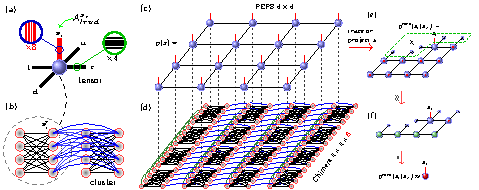
\includegraphics[width=\textwidth]{figures/peps.pdf}
  \caption{Construction of PEPS network} \label{fig:tensors}
\end{figure}

\section{Benchmarks}

To fully investigate the performance of our algorithm, we performed several
benchmarks, testing various metrics quantifying both execution time, as well as
the quality of the found solutions. We tested our algorithm for sets of
\emph{droplet} instances specifically designed to be hard for classical
heuristic solvers, especially ones relying on local updates. We benchmarked our
algorithm against classical solvers based on Parallel-Tempering, and D-Wave
Quantum annealer DW-2000Q$_6$. As it is hard to directly compare samples
obtained from the D-Wave annealer with the output of our deterministic
algorithm, we decided to use time-to-solution as a metric. The time to solution
$\mbox{TTS}$ is defined as:
\begin{equation}
  \label{eq:tts}
  \mbox{TTS} = t \frac{\log(1 - \ptarget)}{\log(1 - \psucc)},
\end{equation}
where $p_{target}$ is the desired probability of obtaining solution, $\psucc$
is the empirical probability of obtaining the solution and $t$ is the running
time of the solver. In addition, for D-Wave annealers, we multiply $\mbox{TTS}$
by the ratio $N/\mbox{num\_qubits}$, to account for the possibility of fitting
multiple instances of the problem on the device at the same time. Naturally,
one might consider $\mbox{TTS}$ metric not only for finding a ground state, but
also for finding a solution approximating a ground state with a given
approximation ratio (i.e. solution lying in the desired lowest fraction of the
full energy spectrum). The results of these benchmarks are presented in Table
\ref{tab:tnvspt}. For all instances, our algorithm was able to find the ground
state, which was not the case for other solvers. However, if one is not
necessarily interested in finding the ground state, both D-Wave annealers and
classical parallel tempering solver might be a better choice, as they were able
to find a satisfying solution in a shorter time. In Fig.
\ref{fig:tn-single-state}, we show an example solution for a single instance
with discreet values of $J_{ij}$ with $dJ=\frac{1}{75}$. One can observe that
increasing the $\beta$ allows for obtaining tighter bounds on the possible
error. It is also visible that the algorithm demonstrates consistency between
the probabilities obtained from the tensor network contractions and the ones
obtained from the Boltzmann weights calculated from the corresponding
configuration energies.

\begin{table}[b]
  \centering
  \begin{tabular}{|l|c|ccc|}
    \hline
    \rowcolor{theader}  Method & approx. ratio & $N=512$   & $N=1152$  & $N=2048$  \\
    \hline
    TN                         & g.s.          & 30s       & 150s      & 450s      \\
    \hline
    \hline
    PT (adaptive)              & g.s.          & 800s      & ---       & ---       \\
    \hline
    PT (geometric)             & $0.01$        & 0.53s     & 4.16s     & ---       \\
    PT (geometric)             & $0.005$       & 2.51s     & 56.4s     & ---       \\
    PT (geometric)             & $0.001$       & 158.4s    & timed-out & ---       \\
    PT (geometric)             & $0.0001$      & 897.6s    & timed-out & ---       \\
    \hline
    \hline
    DWave 2000Q$_6$            & $0.01$        & $0.003$s  & $0.006$s  & $0.02$s   \\
    DWave 2000Q$_6$            & $0.005$       & $0.2$s    & timed-out & timed-out \\
    DWave 2000Q$_6$            & $0.001$       & timed-out & timed-out & timed-out \\
    \hline
    \hline
  \end{tabular}
  \caption{Comparison of time-to-solution metric for our tensor network-based algorithm,
    in-house Parallel Tempering implementation and D-Wave 2000Q$_{6}$. The
    \emph{adaptive} and \emph{geometric} terms refer to the distribution of inverse
    temperature $\beta$ in Parallel Tempering replicas. We bounded the running time
    of our solver to 30 minutes with bond dimension $\chi = 16$, $\beta=3$ and
    probability cutoff $\delta_{p} = 10^{-3}$. For PT, the $t$ in the equation
    \ref{eq:tts} is inferred from the running time and number of performed MC
    sweeps: a single MC sweep took 0.00005s for N=512 and 0.00011s for $N=1024$.
    For the adaptive PT, we used 12 replicas. For geometric PT, we used 25 replicas
    with geometrically distributed $\beta$, with $\beta_{\min}=0.0001$ and
    $\beta_{\max}=10$. For all probabilistic samplers, we used target probability
    $p_{\mbox{target}}=0.99$. In the case of D-Wave annealers, we modified
    instances by dropping inactive qubits. To obtain the reference ground state, we
    once again used our algorithm. We optimized time to solution over annealing
    times of $5\mu s$, $20\mu s$ and $200\mu s$. For each instance and each
    annealing time, we gathered 1000 samples for $N=512$ and 2500 for other values
    of $N$. Also, we used $t=\tau$ for the D-Wave annealers, i.e. we considered
    only annealing time and disregarded other factors contributing to overall
    solution time. This choice is justified by the fact that the other
    contributions are minuscule. The ``timed-out'' string indicates that the given
    algorithm could not find a solution within the given approximation ratio (i.e.
    $\psucc=0$). } \label{tab:tnvspt}
\end{table}

\begin{figure}
  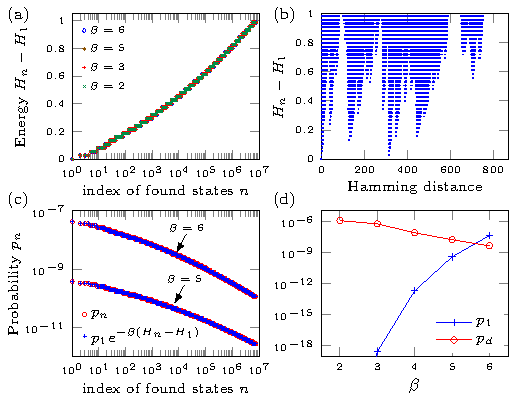
\includegraphics[width=\textwidth]{figures/tn-single-state.pdf}
  \caption{Example result of running our algorithm on a droplet instance with $N=2048$.
    \textbf{a.} Low energy spectrum found by a single run of our algorithm. Observe
    consistency between different values of $\beta$. \textbf{b.} Hamming distance
    of solutions presented in \textbf{a.} from the ground state. \textbf{c.}
    Probabilities of each configuration found for least numerically stable values
    of $\beta$. In the depicted example, we can see full consistency between the
    probabilities obtained from contracting PEPS network $p_{n}$ and the Boltzmann
    weights calculated from the configuration's energy. \textbf{d.} Comparison of
    largest discarded probability $p_{d}$ and the ground state probability $p_{1}$.
    With increasing $\beta$ we were able to achieve $p_{d} < p_{1}$. This indicates
    that the algorithm was indeed able to reach the ground state. }
  \label{fig:tn-single-state}
\end{figure}

We also benchmarked our algorithm on the set of \emph{deceptive cluster loops}
\cite{helmut_deceptive_2018} instances, also expected to be hard for the
classical heuristic solvers. One particular reason for the hardness of these
instances is their enormous ground-state degeneracy. In 97\% of the cases, we
were able to recover the lowest reference energy from
\cite{helmut_deceptive_2018}. In the other 3\% of instances, we were able to
find a better solution.

In our final benchmark, we tested our algorithm with regard to fair sampling.
In order to do so, we solved instances of the Ising model with integer
coefficients and counted the identified ground-state degeneracy. The test
instances had $J_{ij}$ drawn uniformly at random from the set $\{\pm 1, \pm 2,
    \pm 4\}$, following similar tests performed for parallel tempering and parallel
tempering with isoenergetic cluster moves \cite{Zhu_PT+ICM_2015} in Ref.
\cite{zhu_fair_2019}. We present the results in Fig.
\ref{fig:ground-degeneracy}. For smaller system sizes, we observe consistency
with the results reported in \cite{zhu_fair_2019}. For $N=1152$, we observe
some degeneracies approaching the order of $10^{8}$, while the previously
reported numbers were reaching only the magnitude of $10^{6}$. Moreover, we
were able to reach beyond $N=1152$ studied in \cite{zhu_fair_2019}.

\begin{figure}
  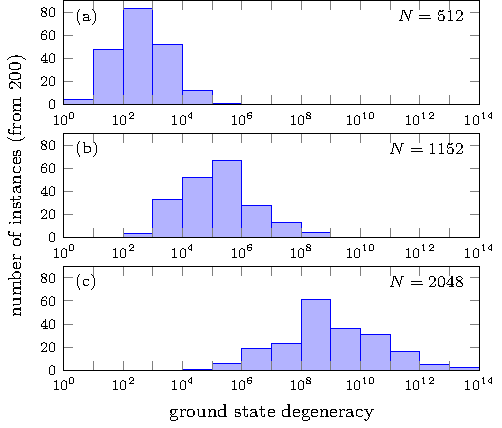
\includegraphics[width=\textwidth]{figures/tn-ground-degeneracy.pdf}
  \caption{Histogram of ground state degeneracy found by our algorithm for test instances
    constructed by drawing couplings $J_{ij}$ uniformly from a set $\{\pm 1, \pm 2,
        \pm 4\}$ and setting all local fields $h_{i} = 0$.}
  \label{fig:ground-degeneracy}
\end{figure}
%%% Local Variables:
%%% mode: latex
%%% TeX-master: "../main"
%%% End:
